\section{Casos de Uso}

\begin{figure}[H]
  \begin{center}
  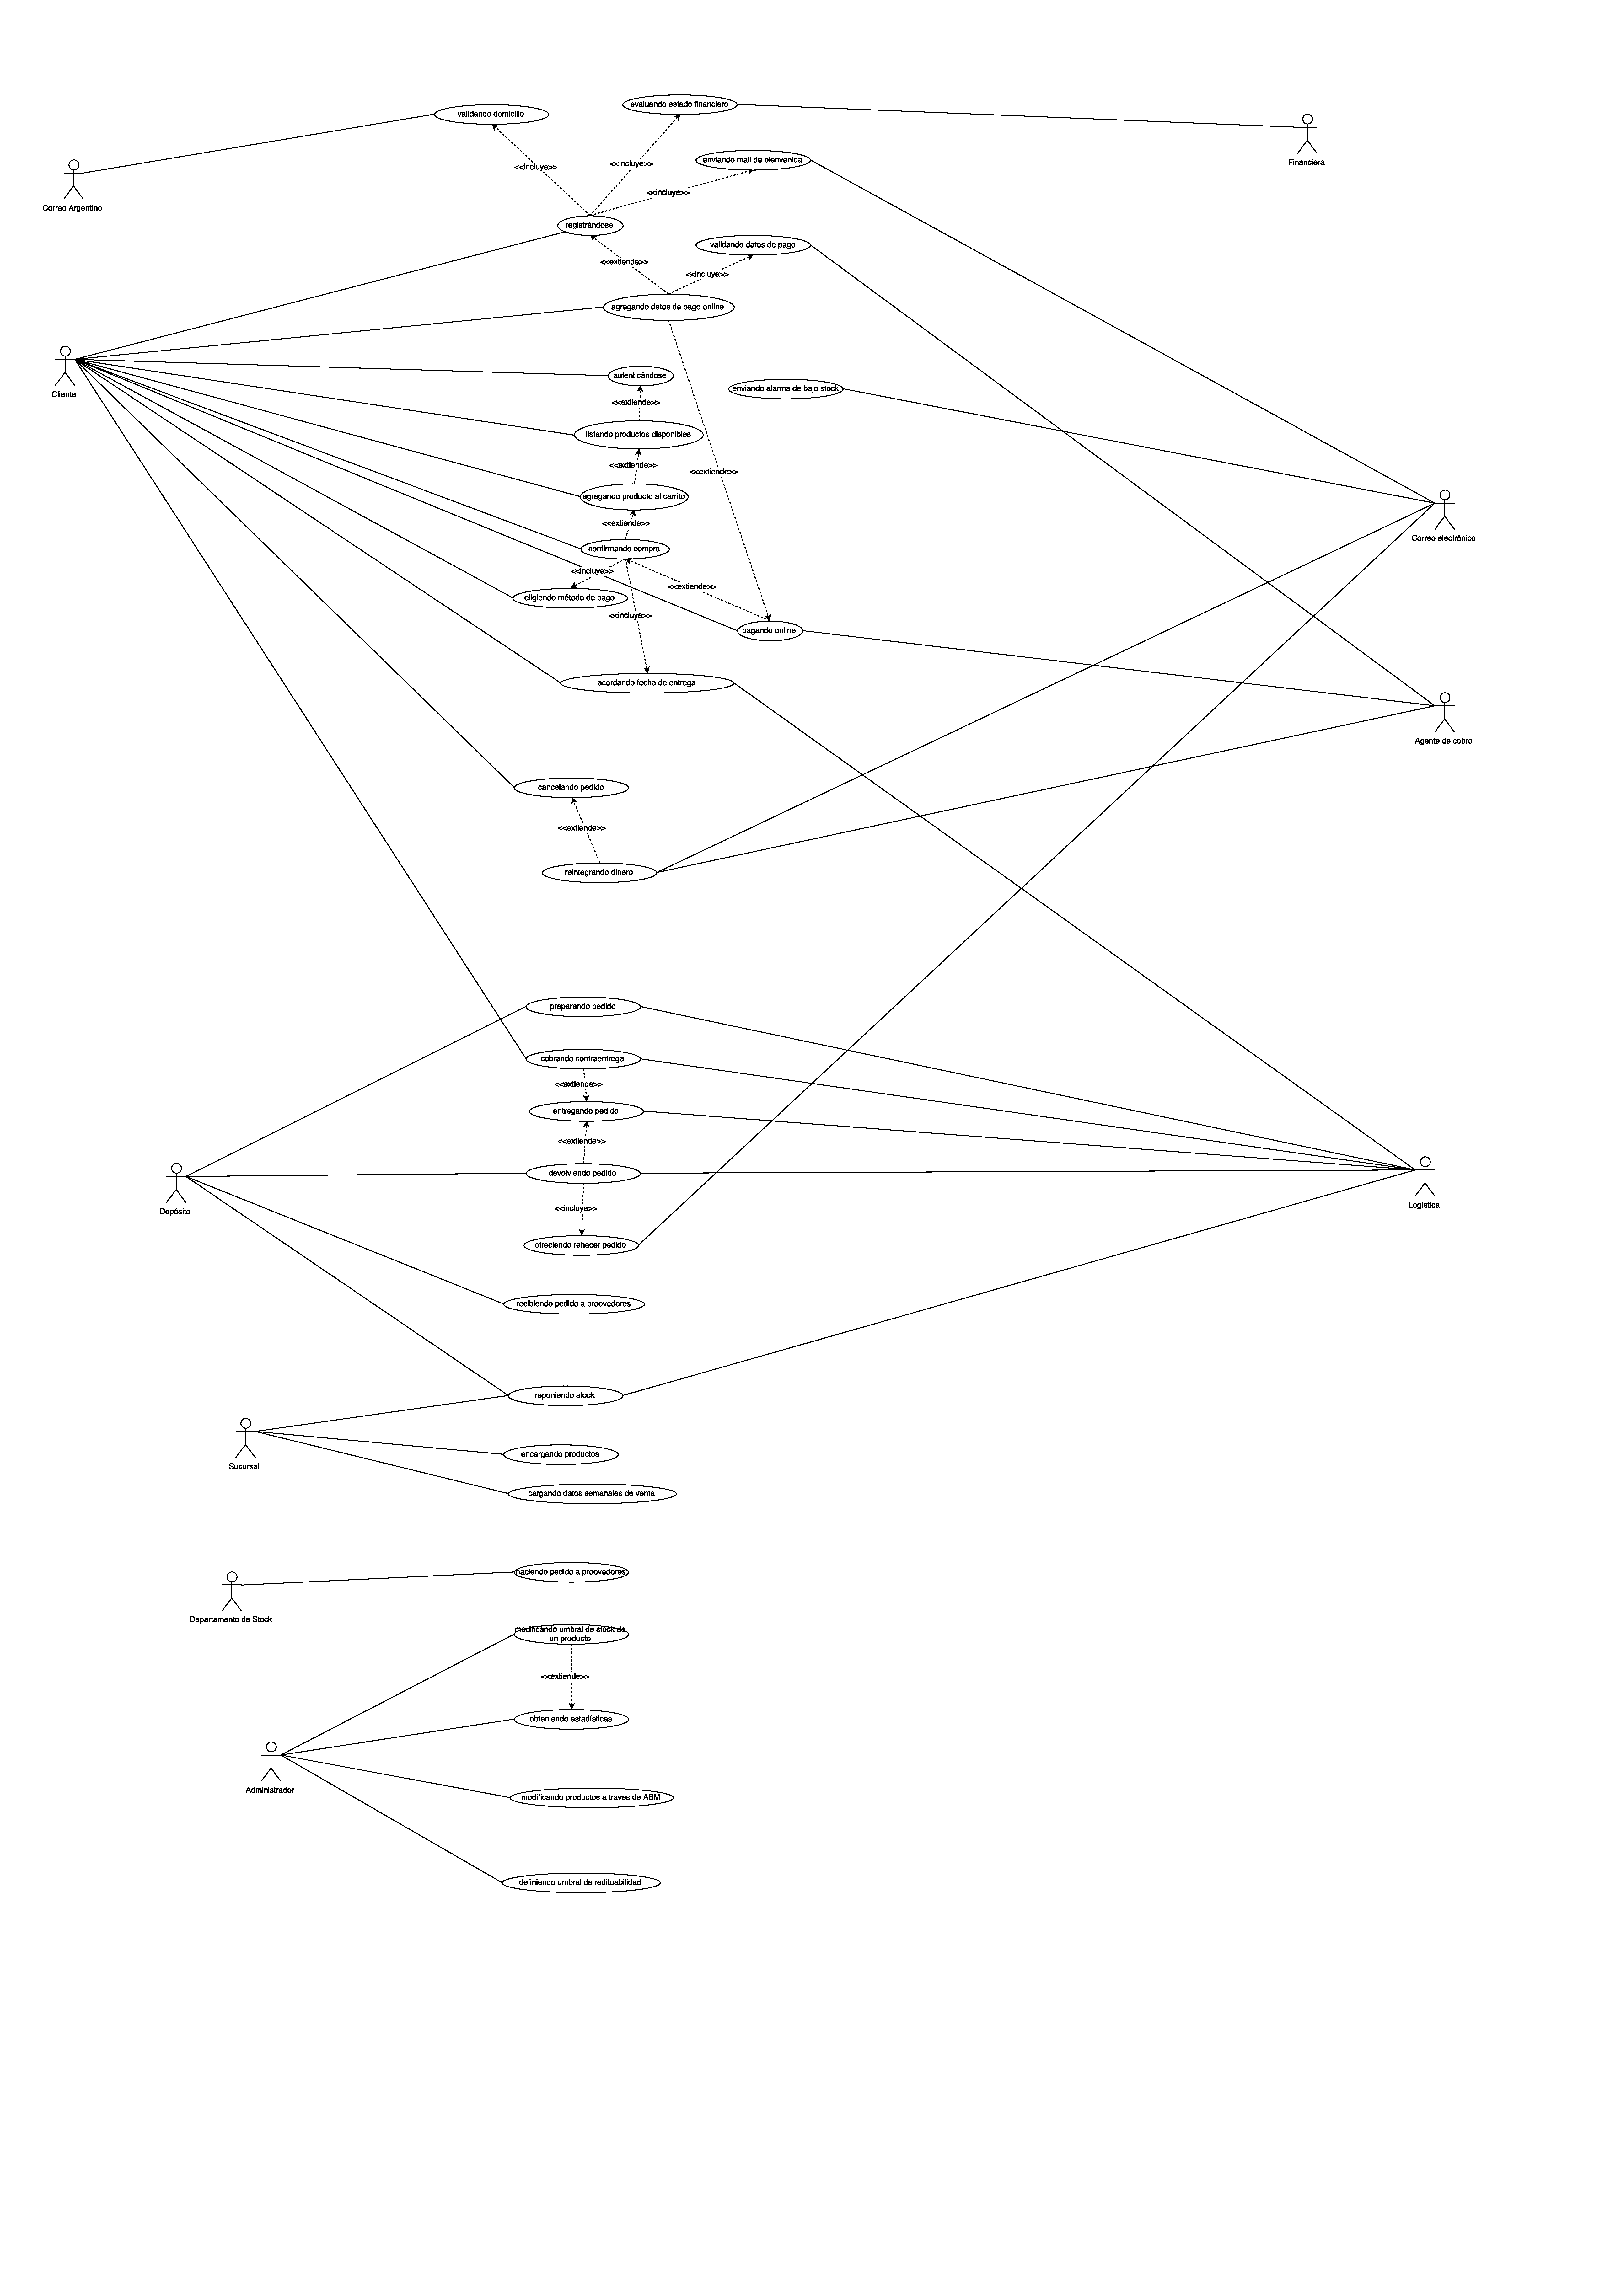
\includegraphics[width=500px]{images/casos-de-uso.pdf}
  \end{center}
\end{figure}

\captionsetup[table]{name=Caso de uso}

\begin{casodeuso}
  \cutitle{Registrándose}
  \cuactors{Cliente}
  \cupost{El cliente se encuentra registrado}
  \cucourse{
  1. El cliente ingresa su usuario y contraseña & \\
  2. El sistema valida que el usuario no exista. & 2.1 Si el usuario ya existe, mostrar mensaje e ir a 1. \\
  3. El sistema valida que la contraseña sea segura. & 3.1 Si la contraseña no es segura, informar al cliente e ir a 1 \\
  4. El cliente ingresa sus datos personales & \\
  5. Incluye CU: evaluando estado financiero & 5.1 Si el cliente tiene deudas, denegarle el registro. FIN CU. \\
  6. El cliente ingresa su dirección & \\
  7. Incluye CU: validando domicilio & 7.1 si el domicilio no es válido, mostrar mensaje e ir a 6.  \\
  8. Si el cliente desea: es extendido por CU: Agregando datos de pago online & \\
  9. El cliente ingresa su mail & \\
  10. Incluye CU: enviando mail de bienvenida & \\
  11. El cliente ingresa al link de bienvenida & 11.1 Si luego de 10 días el usuario no ingresa al link de bienvenida, el registro se cancela, FIN CU.\\
  12. El sistema marca al usuario como validado & \\
  13. FIN CU & \\
  }
  \culabel{Registrandose}
\end{casodeuso}

\begin{casodeuso}
  \cutitle{Evaluando estado financiero}
  \cuactors{Financiera}
  \cucourse{
    1. El sistema envía request a la API de estado financiero con el DNI del cliente & \\
    2. El sistema parsea la respuesta de la API & \\
  }
\end{casodeuso}

\begin{casodeuso}
  \cutitle{Enviando mail de bienvenida}
  \cuactors{Correo electrónico}
  \cucourse{
    1. El sistema define el asunto, cuerpo y destinatario(nuevo cliente) del nuevo mensaje. & \\
    2. El sistema pide al servido de correo electrónico enviar el mensaje. & \\
    3. El servidor de correo electrónico envía el mensaje. & \\
  }
\end{casodeuso}

\begin{casodeuso}
  \cutitle{Autenticándose}
  \cuactors{Cliente}
  \cupost{El cliente se encuentra autenticado}
  \cucourse{
    1. El cliente ingresa el usuario y la contraseña & \\
    2. El sistema verifica los datos ingresados por el cliente & \\
    3. El cliente es redirigido al portal de bienvenida & 3.1 Si los datos son inválidos, se muestra un mensaje de error \\
    4. FIN CU & 4.1 FIN CU\\
  }
  \culabel{Autenticandose}
\end{casodeuso}


\begin{casodeuso}
\cutitle{Listando productos disponibles}
\cuactors{Cliente}
\cupre{El cliente está autenticado}
\cucourse{
1. El cliente ingresa al listado de productos & \\
2. El sistema obtiene los productos que están en stock & \\
3. El sistema obtiene las recomendaciones para el usuario & \\
4. El sistema muestra los productos y las recomendaciones que están en stock & \\
5. Si el cliente lo desea, se extiende con CU: Agregando producto al carrito & \\
6. FIN CU & \\
}
\end{casodeuso}


\begin{casodeuso}
\cutitle{Agregando producto al carrito}
\cuactors{Cliente}
\cupre{El cliente está autenticado}
\cupost{El carrito contiene al producto agregado}
\cucourse{
1. El cliente hace click sobre el producto & \\
2. El sistema muestra un dropdown con la cantidad de unidades que están disponibles en ese momento & \\
3. El cliente elige la cantidad & \\
4. El sistema agrega el producto al carrito y calcula el monto total  & \\
5. Si el cliente lo desea, es extendido por CU: confirmando compra & \\
6. FIN CU & \\
}
\end{casodeuso}


\begin{casodeuso}
\cutitle{Confirmando compra}
\cuactors{Cliente}
\cupre{El cliente tiene un carrito armado}
\cupost{El cliente tiene un carrito reservado y confirmado}
\cucourse{
1. El sistema ratifica la disponibilidad de stock para cada producto, y los reserva para el cliente; el carrito se encuentra reservado &  1.1 Si algún producto ya no tiene disponibilidad, se resta del carrito y se le informa al usuario; vuelve al paso 1. \\
2. Incluye: Calcular costo de envío & \\
3. El sistema informa del costo total de la compra, incluyendo el envío. & \\
4. Incluye: Acordando fecha de entrega & \\
5. Incluye: Eligiendo método de pago & \\
6. Si el pago es online: Es extendido por: Pagando online. & \\
7. El cliente confirma el pedido, FIN CU & 7.1 Si el cliente no confirma el pedido luego de 10 minutos, los productos son reingresados a stock, y el carrito deja de estar reservado, vuelve a paso 1 \\
}
\end{casodeuso}


\begin{casodeuso}
\cutitle{Acordando fecha de entrega}
\cuactors{Cliente, Logística}
\cupre{El cliente tiene un carrito reservado}
\cupost{El pedido tiene fecha tentativa de entrega}
\cucourse{
1. El sistema pregunta próximas fechas libres a la API de logística & \\
2. El sistema presenta las posibles fechas al cliente & \\
3. El cliente elige la fecha deseada & \\
4. FIN CU & \\
}
\end{casodeuso}


\begin{casodeuso}
\cutitle{Eligiendo método de pago}
\cuactors{Cliente}
\cupre{El cliente tiene un carrito reservado}
\cupost{El cliente eligió un método de pago permitido}
\cucourse{
1. El sistema determina si el cliente tiene autorizado el pago contraentrega & \\
2. El sistema presenta los métodos de pagos disponibles & \\
3. El cliente elige el método de pago deseado & \\
4. FIN CU  & \\
}
\end{casodeuso}


\begin{casodeuso}
\cutitle{Pagando online}
\cuactors{Cliente, agente de cobro}
\cupre{El cliente eligió el método de pago online}
\cucourse{
1. Si el cliente lo desea, es extendido por CU: agregando datos de pago online & \\
2. El sistema muestra datos de pago asociados al cliente & \\
3. El cliente indica método y datos de pago & 3.1 Si el cliente no posee datos de pago, ir a paso 1 \\
4. El sistema abre una ventana del agente de cobro con los datos de la transacción. & \\
5. El cliente realiza la operación a través del agente de cobro, generando un token comprobante del pago. & 5.1 Si el agente de cobro rechaza el pago, ir al paso 1.\\
6. El sistema recibe el comprobante de pago, y lo verifica contra el agente de pago. & 6.1 Si el token de pago es inválido, informar al usuario, e ir al paso 1 \\
7. El sistema envía un mail al cliente, informando la compra exitosa y adjuntando un comprobante de pago de la operación a través del sistema de correo electrónico. & \\
8. FIN CU & \\
}
\end{casodeuso}


\begin{casodeuso}
\cutitle{Agregando datos de pago online}
\cuactors{Cliente}
\cupre{El cliente está autenticado}
\cupost{El cliente posee un nuevo dato de pago asociado a su cuenta}
\cucourse{
1. El cliente elige el método de pago online de entre las opciones disponibles & \\
2. Según el método de pago elegido, el cliente ingresa los datos de autenticación solicitados. & \\
3. Incluye: validando datos de pago & \\
4. FIN CU & Si los datos de pago son inválidos regresa a paso 1. \\
}
\end{casodeuso}


\begin{casodeuso}
\cutitle{Cancelando pedido}
\cuactors{Cliente}
\cupre{El cliente tiene un pedido sin confirmar, o confirmado, pero sin armar en depósito.}
\cupost{El pedido es cancelado.}
\cucourse{
1. Si el pedido está sin confirmar, lo cancela, FIN CU. & \\
2. La reserva de productos se anula, y los mismos se reingresan a stock & \\
3. Si fue pagado, es extendido por CU: Reintegrando dinero & \\
4. FIN CU & \\
}
\end{casodeuso}

\begin{casodeuso}
\cutitle{Modificando pedido}
\cuactors{Cliente}
\cupre{El cliente tiene un pedido sin confirmar, o confirmado, pero sin armar en depósito.}
\cupost{El pedido es modificado.}
\cucourse{
1. El cliente quita o agrega los productos que desee, siempre y cuando estén en stock. & \\
2. Si el pedido está sin confirmar, se registra la modificación, FIN CU. & \\
3. Se cancela el pedido anterior: es extendido por CU Cancelando Pedido. & \\
4. Se genera un nuevo pedido con los datos modificados. & \\
5. Es extendido por CU: Confirmando compra. & \\
6. FIN CU & \\
}
\end{casodeuso}

\begin{casodeuso}
\cutitle{Validando datos de pago}
\cuactors{Agente de cobro}
\cupre{El cliente ingresó los datos de pago}
\cupost{Los datos de pago fueron validados}
\cucourse{
1. El sistema contrasta los datos de pago del cliente contra el agente de cobro correspondiente a través de una API. & \\
2. FIN CU & 2.1 Si los datos de pago no son válidos, el sistema los marca como inválidos, FIN CU\\
}
\end{casodeuso}



\begin{casodeuso}
\cutitle{Reintegrando dinero}
\cuactors{Agente de cobro, Correo electrónico}
\cupre{El cliente canceló un pedido}
\cupost{El dinero correspondiente al pedido fue reintegrado al cliente}
\cucourse{
1. El sistema contacta al agente de cobro, solicitando la anulación de las operaciones correspondientes al pago del pedido. & \\
2. El agente de cobro anula las operaciones de pago solicitadas, y entrega un número de operación y un comprobante de anulación para cada una de ellas. & \\
3. El sistema envía un mail al cliente, informando que el pedido fue anulado, a través del sistema de correo electrónico, adjuntando los comprobantes de pago & 3.1 Si el pago no puede ser anulado, se le informa de la situación al cliente, brindándole los números de operación.\\
4. FIN CU & \\
}
\end{casodeuso}


\begin{casodeuso}
\cutitle{Validando domicilio}
\cuactors{Correo argentino}
\cupre{El cliente ingresó los datos de su domicilio}
\cupost{Los datos de su domicilio fueron validados}
\cucourse{
1. El sistema verifica los datos de domicilio del cliente mediante la API del Correo Argentino & \\
2. FIN CU & 2.1 Si los datos de domicilio no son correctos, se marcan como inválidos. FIN CU \\
}
\end{casodeuso}


\begin{casodeuso}
\cutitle{Preparando pedido}
\cuactors{Depósito, Logística}
\cupre{El cliente tiene un pedido confirmado}
\cupost{El cliente tiene un pedido preparado}
\cucourse{
1. El sistema brinda el listado de  productos a preparar, junto con el domicilio y la fecha y hora de entrega & \\
2. Un operario del depósito marca el pedido como preparado y se encarga de empaquetar los productos & \\
3. Depósito informa del pedido a logística, y se pacta el envío para la fecha correspondiente; los datos de la operación se cargan en el sistema & \\
4. La información correspondiente al envío: remito, hoja de ruta, factura, etcétera, se empaqueta junto con el mismo. &  \\
5. FIN CU & \\
}
\end{casodeuso}


\begin{casodeuso}
\cutitle{Entregando pedido}
\cuactors{Logística, Depósito}
\cupre{El cliente tiene un pedido preparado}
\cupost{Se realiza un intento de entrega}
\cucourse{
1. Logística retira el pedido. & \\
2. Logística entrega el pedido al cliente. & 2.1 Si el cliente no recibe el pedido, es extendido por CU: Devolviendo pedido.\\
3. Si el pago es contraentrega, es extendido por CU: Cobrando contraentrega & \\
4. Logística registra la entrega al cliente satisfactoria & \\
5. FIN CU. & \\
}
\end{casodeuso}


\begin{casodeuso}
\cutitle{Cobrando contraentrega}
\cuactors{Logística, Cliente}
\cupre{El cliente eligió contraentrega como método de pago}
\cupost{El pago del pedido fue efectuado}
\cucourse{
1. El transportista presenta la factura de compra & \\
2. El cliente entrega el dinero correspondiente & \\
3. FIN CU & \\
}
\end{casodeuso}


\begin{casodeuso}
\cutitle{Devolviendo pedido}
\cuactors{Logística, Depósito}
\cupre{La entrega del pedido fue fallida}
\cupost{El pedido está anulado y los productos aprobados fueron reingresados a stock}
\cucourse{
1. Logística devuelve stock al depósito & \\
2. Encargados del depósito hacen un inventario de la mercadería malograda & \\
3. La mercadería en buen estado es reingresada a stock & \\
4. Depósito carga la falta del cliente y el costo generado a la empresa & \\
5. El pedido es anulado. & \\
6. Incluye: Ofreciendo rehacer pedido. & \\
7. FIN CU & \\
}
\end{casodeuso}

\begin{casodeuso}
\cutitle{Ofreciendo rehacer pedido}
\cuactors{Correo electrónico}
\cupre{El cliente tiene un pedido anulado.}
\cupost{Se le ofrece al cliente rehacer el pedido.}
\cucourse{
1. El sistema genera un link hacia una orden de compra con el mismo carrito del pedido anulado & \\
2. El sistema de correo electrónico envía un mail al cliente con el link y una invitación a rehacer el pedido & \\
3. FIN CU & \\
}
\end{casodeuso}



\begin{casodeuso}
\cutitle{Enviando alarma de bajo stock}
\cuactors{Correo electronico}
\cupre{Existe al menos un producto con stock menor al límite estipulado}
\cupost{Se avisa de la falta de stock al Departamento de Stock}
\cucourse{
1. El sistema prepara una lista de todos los productos por debajo del límite estipulado y el stock necesario para reestablecerlos & \\
2. El sistema de correo electrónico envía un mail con los datos al Departamento de Stock & \\
3. FIN CU & \\
}
\end{casodeuso}


\begin{casodeuso}
\cutitle{Haciendo pedido a proveedores}
\cuactors{Departamento de stock}
\cupre{Una alarma de bajo stock fue activada}
\cupost{Se realiza un nuevo pedido a un proveedor}
\cucourse{
1. El Departamento de Stock determina al mejor proveedor y efectúa una compra & \\
2. El Departamento de Stock carga el comprobante de pedido  al sistema & \\
3. FIN CU & \\
}
\end{casodeuso}

\begin{casodeuso}
\cutitle{Recibiendo pedido a proveedores}
\cuactors{Depósito}
\cupost{La mercadería es ingresada al depósito}
\cucourse{
1. Empleados del depósito guardan la mercadería & \\
2. Depósito registra el ingreso y el sistema actualiza el stock de los nuevos productos & \\
3. FIN CU & \\
}
\end{casodeuso}

\begin{casodeuso}
\cutitle{Reponiendo stock}
\cuactors{Depósito, Logística, Sucursal}
\cupre{Hay un pedido de reposición de la sucursal}
\cupost{Los productos requeridos son ingresados a la sucursal}
\cucourse{
1. Depósito reserva todo el stock necesario para completar el pedido, o el máximo posible en caso de que la reserva de stock sea menor a esta cantidad, informando la baja de los productos correspondientes. & 1.1 Si no se ha reservado el stock necesario para el pedido, se espera a que llegue una reposición y se vuelve a 1 \\
2. Un empleado del depósito empaqueta los productos reservados y avisa a logística  & \\
3. Depósito entrega el pedido a logística junto con una hoja de ruta & \\
4. Logística transporta el envío hasta la sucursal & \\
5. La sucursal repone los productos en las góndolas & \\
6. FIN CU & \\
}
\end{casodeuso}



\begin{casodeuso}
\cutitle{Definiendo umbral de redituabilidad}
\cuactors{Administrador}
\cupost{Se redefine el umbral de redituabilidad}
\cucourse{
1. El administrador ingresa el nuevo umbral de redituabilidad & \\
2. El sistema guarda el nuevo umbral & \\
3. FIN CU & \\
}
\end{casodeuso}


\begin{casodeuso}
\cutitle{Modificando productos a través de ABM}
\cuactors{Administrador}
\cupost{Los productos solicitados son modificados}
\cucourse{
1. El sistema muestra una interfaz para agregar, dar de baja, y modificar productos & \\
2. El administrador ingresa la operación requerida & \\
3. El sistema realiza los cambios necesarios y confirma la operación & \\
4. FIN CU & \\
}
\end{casodeuso}

\begin{casodeuso}
\cutitle{Obteniendo estadísticas}
\cuactors{Administrador}
\cupost{Se envían las estadísticas al administrador}
\cucourse{
1. El administrador solicita las estadísticas a través del sistema & \\
2. El sistema genera las estadísticas de venta de cada producto y compras de cada usuario, y las prepara para su adecuada visualización & \\
3. El administrador descarga las estadísticas a través del sistema & \\
4. Si administrador desea modificar límite de productos, es extendido por CU: Modificando umbral de stock de un producto. & \\
5. FIN CU. & \\
}
\end{casodeuso}


\begin{casodeuso}
\cutitle{Modificando umbral de stock de un producto}
\cuactors{Administrador}
\cupre{El producto existe}
\cupost{El producto tiene un nuevo umbral de stock}
\cucourse{
1. El administrador informa del nuevo límite para el producto & \\
2. FIN CU & \\
}
\end{casodeuso}


\begin{casodeuso}
\cutitle{Encargando productos}
\cuactors{Sucursal, Depósito}
\cupre{La sucursal está autenticada, desea encargar productos}
\cupost{Los productos deseados fueron encargados}
\cucourse{
1. La sucursal ingresa el listado de productos que desea encargar. & \\
2. El sistema informa a depósito del pedido. & \\
3. El sistema le confirma a la sucursal que el pedido fue encargado. & \\
4. FIN CU & \\
}
\end{casodeuso}

\begin{casodeuso}
\cutitle{Cargando datos semanales de venta}
\cuactors{Sucursal}
\cupre{La sucursal tiene datos de venta para informar}
\cupost{El sistema contiene datos de venta actualizados}
\cucourse{
1. La sucursal carga los datos de venta de la semana a través de una interfaz sencilla, por ejemplo una planilla de cálculos. & \\
2. El sistema procesa los datos de venta, y los integra a su base de estadísticas & \\
3. FIN CU & \\
}
\end{casodeuso}
